%----------------------------------------------------------------------------------------
%	CHAPTER 10
%----------------------------------------------------------------------------------------
\chapterimage{ChapterImages/chapter10.png} % Chapter heading image

\chapter{Inter-Process Communication (IPC)}
\label{ch:ipc}

\section{Introduction}
By default, modern operating systems isolate processes from one another. Each process has its own independent memory address space, ensuring that a bug or crash in one program cannot easily corrupt the data of another. However, many applications require processes to work together -- for instance, the parent/child pairs you built with \texttt{fork()} in Chapter~\ref{ch:processes}, or the threads from Chapter~\ref{ch:multithreading} (which, unlike processes, already share memory by default and so need IPC far less often).

Inter-Process Communication (IPC) is a set of mechanisms that allows separate processes to exchange data safely and in a structured manner across these isolated boundaries. IPC is essential for cooperating processes, parallel tasks, and any system that requires controlled data sharing.

In the context of execution, processes are either:
\begin{itemize}
    \item \textbf{Independent processes:} they share no data and operate in complete isolation; they do not need IPC.
    \item \textbf{Cooperating processes:} they interact, synchronize, and share data; they require IPC mechanisms to function.
\end{itemize}

Linux provides several IPC mechanisms, each suited to different types of communication. In this chapter, we will explore Pipes, FIFOs, Message Queues, Shared Memory, Signals, and Sockets. Figure~\ref{fig:ipc-data-paths} previews the key distinction that runs through most of this chapter: whether data passes \emph{through} the kernel, or whether processes reach the same memory \emph{directly}.

\begin{figure}[h]
    \centering
    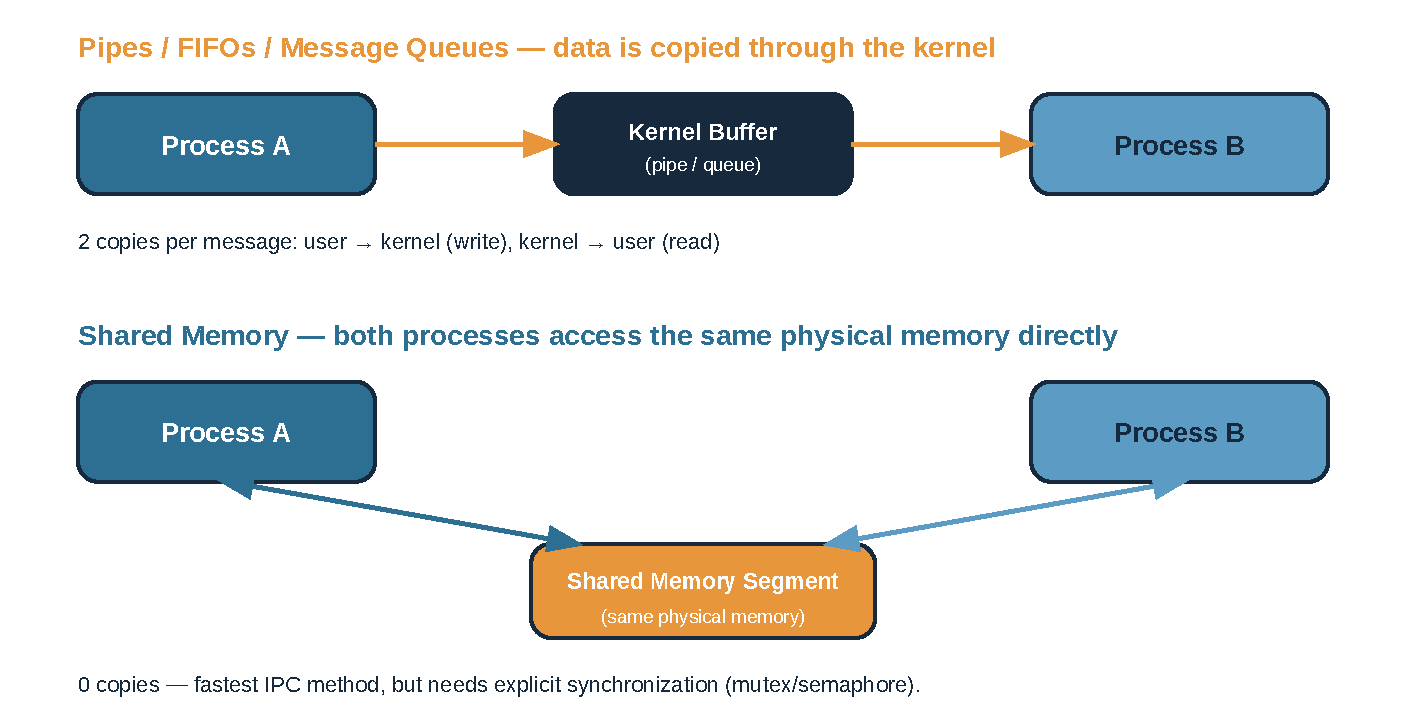
\includegraphics[width=\textwidth]{Images/Chapter10/ipc-data-paths.pdf}
    \caption{Two fundamentally different data paths: kernel-mediated (pipes, FIFOs, message queues) versus direct shared memory.}
    \label{fig:ipc-data-paths}
\end{figure}

\section{Pipes (Anonymous Pipes)}
A pipe is one of the oldest and simplest inter-process communication methods in Unix-like operating systems. Pipes allow a process to transfer a stream of bytes unidirectionally from one point (the writer) to another point (the reader).

Because anonymous pipes only exist in memory and lack a name in the file system, they can \textbf{only} be used between related processes (typically a parent and its child). Furthermore, this method is \textbf{volatile}: once the processes terminate, the pipe and any unread data are permanently destroyed.

\begin{table}[h!]
\centering
\small
\renewcommand{\arraystretch}{1.3}
\begin{tabular}{|p{5.5cm}|p{8.5cm}|}
\hline
\textbf{Function / System Call} & \textbf{Description} \\ \hline
\texttt{pipe(int fd[2])} & Creates a pipe. \texttt{fd[0]} is the read end; \texttt{fd[1]} is the write end. \\ \hline
\texttt{fork(void)} & Creates a child process that inherits the pipe's file descriptors. \\ \hline
\texttt{write(int fd, const void *buf, size\_t count)} & Writes \texttt{count} bytes from \texttt{buf} to the pipe. \\ \hline
\texttt{read(int fd, void *buf, size\_t count)} & Reads up to \texttt{count} bytes from the pipe into \texttt{buf}. \\ \hline
\texttt{close(int fd)} & Closes a file descriptor. Always close unused ends of a pipe! \\ \hline
\end{tabular}
\caption{System Calls used for Anonymous Pipes}
\end{table}

Figure~\ref{fig:pipe-fd-flow} shows how the file descriptors from \texttt{pipe()} are used after \texttt{fork()}: both processes inherit both ends, but each immediately closes the end it doesn't need.

\begin{figure}[h]
    \centering
    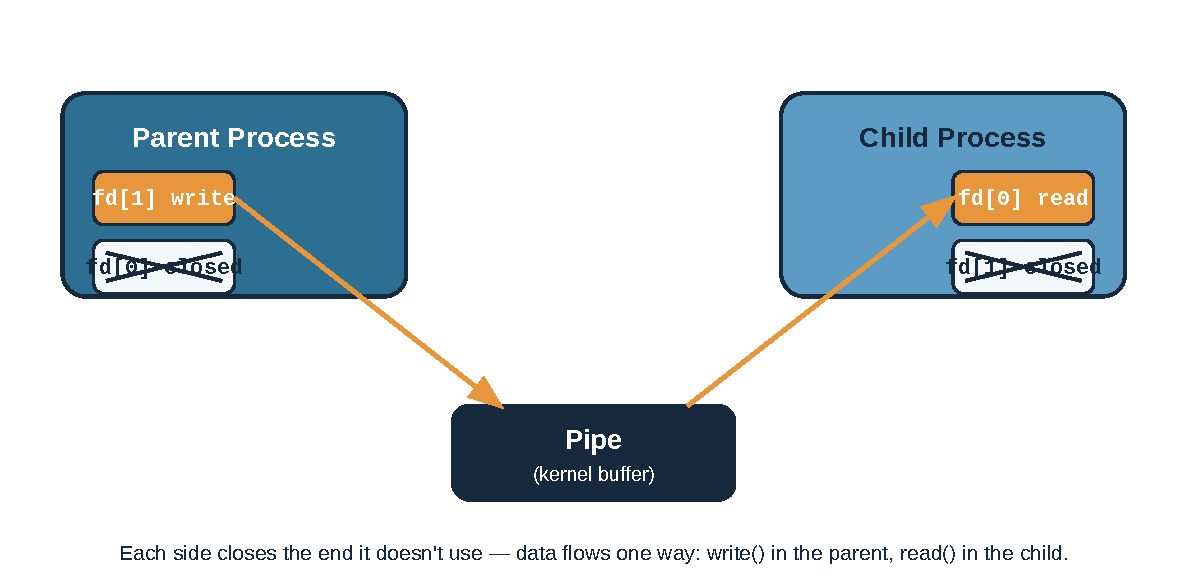
\includegraphics[width=0.85\textwidth]{Images/Chapter10/pipe-fd-flow.pdf}
    \caption{After \texttt{fork()}, the parent keeps \texttt{fd[1]} (write) and the child keeps \texttt{fd[0]} (read); the unused end on each side is closed.}
    \label{fig:pipe-fd-flow}
\end{figure}

\textbf{Example Code: Parent writing to Child}
\begin{lstlisting}[language=C]
#include <stdio.h>
#include <stdlib.h>
#include <unistd.h>
#include <string.h>
#include <sys/wait.h>

int main() {
    int fd[2];
    pid_t pid;
    char buffer[100];

    // Create the pipe
    if (pipe(fd) == -1) {
        perror("pipe failed");
        exit(1);
    }

    // Fork to create child process
    pid = fork();

    if (pid < 0) {
        perror("fork failed");
        exit(1);
    }

    if (pid > 0) {  // Parent process
        close(fd[0]);  // Close unused read end

        // Write message to the pipe
        char *msg = "Message from parent!";
        write(fd[1], msg, strlen(msg) + 1);  // +1 to include null terminator

        close(fd[1]);  // Close write end

        // Wait for child to finish
        wait(NULL);
        printf("Parent: Message sent successfully.\n");
    }
    else {  // Child process
        close(fd[1]);  // Close unused write end

        // Read message from the pipe
        read(fd[0], buffer, sizeof(buffer));

        printf("Child received: %s\n", buffer);

        close(fd[0]);  // Close read end
    }

    return 0;
}
\end{lstlisting}

\textbf{Step-by-Step Explanation:}
\begin{itemize}
    \item \texttt{pipe(fd)} creates the communication channel \emph{before} the fork.
    \item \texttt{fork()} duplicates the process. Now both parent and child have access to \texttt{fd[0]} and \texttt{fd[1]}.
    \item Data flows in one direction. To enforce this, the parent closes its read end (\texttt{fd[0]}), and the child closes its write end (\texttt{fd[1]}).
    \item The parent uses \texttt{write()} to push the string into the pipe, while the child uses \texttt{read()} to pull it out.
\end{itemize}

\section{FIFOs (Named Pipes)}
A FIFO (First-In, First-Out) is a type of pipe that possesses a specific, visible name in the file system. Unlike a normal (anonymous) pipe, which is temporary and restricted to related processes, a FIFO allows completely unrelated processes -- even ones started from separate terminals, with no parent/child relationship at all -- to communicate, as long as they have the appropriate file permissions.

A FIFO's data still lives in an in-memory kernel buffer, exactly like an anonymous pipe (it is \emph{not} written to disk); only its \emph{name} is visible in the file system. Processes interact with it using standard file operations: \texttt{open()}, \texttt{read()}, \texttt{write()}, and \texttt{close()}.

\begin{table}[h!]
\centering
\small
\renewcommand{\arraystretch}{1.3}
\begin{tabular}{|p{5.5cm}|p{8.5cm}|}
\hline
\textbf{Function / Command} & \textbf{Description} \\ \hline
\texttt{mkfifo(const char *path, mode\_t mode)} & Creates a FIFO special file at \texttt{path} (C function). \\ \hline
\texttt{mkfifo path} & Same, from the shell -- no compilation needed. \\ \hline
\texttt{open(const char *path, int flags)} & Opens the FIFO for reading or writing; blocks until the other end is also opened. \\ \hline
\texttt{read()} / \texttt{write()} & Same semantics as an anonymous pipe, once both ends are open. \\ \hline
\texttt{unlink(const char *path)} & Removes the FIFO's name from the file system. \\ \hline
\end{tabular}
\caption{Functions and Commands used for FIFOs}
\end{table}

\textbf{Example: Two Independent Programs, One FIFO}\\
Unlike a pipe, a FIFO is naturally demonstrated with two \emph{separate} programs run in two separate terminals.

\texttt{writer.c}:
\begin{lstlisting}[language=C]
#include <stdio.h>
#include <fcntl.h>
#include <string.h>
#include <unistd.h>

int main() {
    mkfifo("myfifo", 0666);  // Create the FIFO (harmless if it already exists)

    int fd = open("myfifo", O_WRONLY);  // Blocks until a reader opens it too
    char *msg = "Hello through a FIFO!";
    write(fd, msg, strlen(msg) + 1);
    close(fd);

    printf("Writer: message sent.\n");
    return 0;
}
\end{lstlisting}

\texttt{reader.c}:
\begin{lstlisting}[language=C]
#include <stdio.h>
#include <fcntl.h>
#include <unistd.h>

int main() {
    mkfifo("myfifo", 0666);  // Create the FIFO (harmless if it already exists)

    int fd = open("myfifo", O_RDONLY);  // Blocks until a writer opens it too
    char buffer[100];
    read(fd, buffer, sizeof(buffer));
    close(fd);

    printf("Reader received: %s\n", buffer);
    return 0;
}
\end{lstlisting}

\textbf{Running it:}
\begin{lstlisting}[language=Terminal]
$ gcc reader.c -o reader
$ gcc writer.c -o writer
$ ./reader &        # start the reader first, in the background
$ ./writer           # then run the writer
\end{lstlisting}
\textbf{Note:} \texttt{open()} on a FIFO blocks until \emph{both} a reader and a writer have opened it -- this is why running the reader first (with \texttt{\&}, so it doesn't block your terminal) and the writer second works cleanly.

\section{System V Message Queues}
Message queues allow processes to send and receive structured messages rather than just an unstructured stream of bytes. These queues are stored inside the operating system kernel and act as persistent buffers for messages until they are explicitly deleted.

Unlike pipes, messages in a queue are structured into a \textbf{message type} and \textbf{message text}. This allows the receiving process to selectively pull messages based on their type, rather than strictly receiving them in the order they were sent (FIFO).

\begin{table}[h!]
\centering
\small
\renewcommand{\arraystretch}{1.4}
\begin{tabular}{|p{6.5cm}|p{7.5cm}|}
\hline
\textbf{Function} & \textbf{Description} \\ \hline
\texttt{msgget(key\_t key, int msgflg)} & Creates a new message queue or accesses an existing one based on the \texttt{key}. \\ \hline
\texttt{msgsnd(int msgid, const void *msgp, size\_t msgsz, int msgflg)} & Appends a message to the queue. \\ \hline
\texttt{msgrcv(int msgid, void *msgp, size\_t msgsz, long mtype, int msgflg)} & Receives a message from the queue, filtered by \texttt{mtype}. \\ \hline
\texttt{msgctl(int msgid, int cmd, struct msqid\_ds *buf)} & Performs control operations (e.g., \texttt{IPC\_RMID} to remove the queue). \\ \hline
\end{tabular}
\caption{System V Message Queue Functions}
\end{table}

\textbf{Example Code: Typed Message Passing}
\begin{lstlisting}[language=C]
#include <stdio.h>
#include <stdlib.h>
#include <string.h>
#include <sys/ipc.h>
#include <sys/msg.h>
#include <unistd.h>
#include <sys/wait.h>

// Message buffer structure (mtype must be first and of type long)
struct msgbuf {
    long mtype;          // Message type
    char mtext[100];     // Message text/data
};

int main() {
    key_t key;
    int msgid;
    struct msgbuf message;

    // Generate a unique key using ftok (requires a file named "msgfile" to exist)
    key = ftok("msgfile", 65);
    if (key == -1) {
        perror("ftok failed");
        exit(1);
    }

    // Create or get the message queue
    msgid = msgget(key, 0666 | IPC_CREAT);
    if (msgid == -1) {
        perror("msgget failed");
        exit(1);
    }

    pid_t pid = fork();

    if (pid > 0) {
        // Parent process - Sender
        message.mtype = 1;
        strcpy(message.mtext, "Hello from System V Message Queue!");

        if (msgsnd(msgid, &message, strlen(message.mtext) + 1, 0) == -1) {
            perror("msgsnd failed");
            exit(1);
        }

        printf("Parent: Message sent successfully.\n");

        // Wait for child to finish
        wait(NULL);

        // Remove the message queue
        msgctl(msgid, IPC_RMID, NULL);
        printf("Message queue removed.\n");
    }
    else if (pid == 0) {
        // Child process - Receiver
        sleep(1);  // Give parent time to send first

        // Note: mtype = 1 means it will only grab messages of type 1
        if (msgrcv(msgid, &message, sizeof(message.mtext), 1, 0) == -1) {
            perror("msgrcv failed");
            exit(1);
        }

        printf("Child received: %s\n", message.mtext);
    }
    else {
        perror("fork failed");
        exit(1);
    }

    return 0;
}
\end{lstlisting}
\textbf{Note:} For \texttt{ftok} to work successfully in this example, a file named \texttt{"msgfile"} must exist in the same directory where the program is executed. You can create it using \texttt{touch msgfile} before running the code.

\section{System V Shared Memory}
Shared memory is an IPC mechanism that maps a specific segment of physical memory into the address spaces of multiple processes. Because data is written directly to memory rather than copied through the kernel via system calls (like pipes or queues), it is the \textbf{fastest} method of data transfer between processes -- the bottom panel of Figure~\ref{fig:ipc-data-paths} shows why: there is no intermediate kernel buffer to copy through at all.

\textbf{Important Warning:} Because shared memory allows simultaneous access by multiple processes, it inherently introduces race conditions, in exactly the same way concurrent threads did in Chapter~\ref{ch:multithreading}. This method requires \textbf{synchronization}. Mechanisms such as Mutexes or Semaphores must be used to control access and ensure data consistency. (In the educational example below, a simple \texttt{sleep()} is used to delay the child, but this is unsafe for real-world applications).

\begin{table}[h!]
\centering
\small
\renewcommand{\arraystretch}{1.4}
\begin{tabular}{|p{6.5cm}|p{7.5cm}|}
\hline
\textbf{Function} & \textbf{Description} \\ \hline
\texttt{ftok(const char *pathname, int proj\_id)} & Generates a unique key for System V IPC using an existing file. \\ \hline
\texttt{shmget(key\_t key, size\_t size, int shmflg)} & Creates a new shared memory segment or accesses an existing one. \\ \hline
\texttt{shmat(int shmid, const void *shmaddr, int shmflg)} & Attaches the shared memory segment to the calling process's address space. \\ \hline
\texttt{shmdt(const void *shmaddr)} & Detaches the shared memory segment from the process. \\ \hline
\texttt{shmctl(int shmid, int cmd, struct shmid\_ds *buf)} & Performs control operations on shared memory (e.g., \texttt{IPC\_RMID} to remove). \\ \hline
\end{tabular}
\caption{System V Shared Memory Functions}
\end{table}

\textbf{Example Code: Writer and Reader via Shared Memory}
\begin{lstlisting}[language=C]
#include <stdio.h>
#include <stdlib.h>
#include <unistd.h>
#include <sys/ipc.h>
#include <sys/shm.h>
#include <sys/wait.h>
#include <string.h>

#define SHM_SIZE 100

int main() {
    key_t key;
    int shmid;
    char *data;

    // Generate unique key (requires "shmfile.txt" to exist)
    key = ftok("shmfile.txt", 65);
    if (key == -1) {
        perror("ftok failed");
        exit(1);
    }

    // Create shared memory segment
    shmid = shmget(key, SHM_SIZE, 0666 | IPC_CREAT);
    if (shmid == -1) {
        perror("shmget failed");
        exit(1);
    }

    pid_t pid = fork();

    if (pid < 0) {
        perror("fork failed");
        exit(1);
    }

    if (pid > 0) {  // Parent process (Writer)
        // Attach to shared memory
        data = (char *) shmat(shmid, NULL, 0);
        if (data == (char *) -1) {
            perror("shmat failed");
            exit(1);
        }

        // Write message to shared memory
        strcpy(data, "Hello from Parent using ftok & shm!");

        printf("Parent wrote: %s\n", data);

        // Detach from process space
        shmdt(data);

        // Wait for child to finish reading
        wait(NULL);

        // Remove shared memory
        shmctl(shmid, IPC_RMID, NULL);
        printf("Shared memory removed.\n");
    }
    else {  // Child process (Reader)
        sleep(1);  // Educational hack to ensure parent writes first

        // Connect using the same key
        key = ftok("shmfile.txt", 65);
        shmid = shmget(key, SHM_SIZE, 0666);

        // Attach to shared memory
        data = (char *) shmat(shmid, NULL, 0);

        // Read and print
        printf("Child read: %s\n", data);

        // Detach
        shmdt(data);
    }

    return 0;
}
\end{lstlisting}

\section{Signals}
A signal is a very simple, lightweight, asynchronous message used to control or synchronize the behavior of a process. No complex data payload is transferred via a signal; it is primarily used to tell another process \textbf{``do something''} or \textbf{``stop.''} Despite the lack of data payload, it is still categorized as IPC because it alters process execution and allows minimal communication.

Operating systems use signals internally (e.g., stopping a process for an invalid memory access), and users invoke them regularly via the terminal -- every time you press \texttt{Ctrl+C} to stop a running program, you are sending it a signal.

\begin{table}[h!]
\centering
\small
\renewcommand{\arraystretch}{1.4}
\begin{tabular}{|p{6cm}|p{2.5cm}|p{5.5cm}|}
\hline
\textbf{Description} & \textbf{Signal} & \textbf{Default Action} \\ \hline
Terminal interrupt (Ctrl+C by user) & \texttt{SIGINT} & Terminate process \\ \hline
Terminal hangup (e.g., modem disconnect) & \texttt{SIGTERM} & Terminate process gracefully \\ \hline
Kill (cannot be caught or ignored) & \texttt{SIGKILL} & Terminate process immediately \\ \hline
User-defined signal 1 & \texttt{SIGUSR1} & Developer-defined behavior \\ \hline
\end{tabular}
\caption{Common Unix/Linux Signals}
\end{table}

\textbf{Catching a Signal in C}\\
Most signals can be intercepted with a custom \emph{handler} function using \texttt{signal()}, instead of letting the default action (usually termination) happen. \texttt{SIGKILL} is the one notable exception -- it can never be caught, blocked, or ignored, which is exactly why it is used as a last resort.
\begin{lstlisting}[language=C]
#include <stdio.h>
#include <signal.h>
#include <unistd.h>

// This function runs instead of the default action when SIGUSR1 arrives
void handle_sigusr1(int sig) {
    printf("Caught signal %d (SIGUSR1)! Doing custom cleanup...\n", sig);
}

int main() {
    signal(SIGUSR1, handle_sigusr1);  // Register our handler

    printf("PID = %d. Waiting for a SIGUSR1 signal...\n", getpid());
    while (1) {
        pause();  // Sleep until any signal arrives
    }

    return 0;
}
\end{lstlisting}

\textbf{Sending the signal from another terminal:}
\begin{lstlisting}[language=Terminal]
$ kill -SIGUSR1 <PID>
\end{lstlisting}
\textbf{Step-by-Step Explanation:}
\begin{itemize}
    \item \texttt{signal(SIGUSR1, handle\_sigusr1)} tells the kernel to run \texttt{handle\_sigusr1} instead of terminating the process when \texttt{SIGUSR1} arrives.
    \item \texttt{pause()} puts the process to sleep until \emph{any} signal is delivered -- it does no polling, so it costs no CPU while waiting.
    \item The \texttt{kill} command, despite its name, just \emph{sends a signal} -- by default \texttt{SIGTERM}, but any signal (including a harmless one like \texttt{SIGUSR1}) can be specified.
    \item After the handler function returns, execution resumes right where it left off -- back inside \texttt{pause()}, which then loops around to \texttt{pause()} again.
\end{itemize}

\section{Sockets}
Sockets are one of the most advanced IPC methods available. While all previous methods restrict communication to processes running on the same physical machine, sockets allow data exchange between two processes regardless of whether they are on the same machine (\textbf{Unix Domain Sockets}) or across different machines in a network (\textbf{Internet Sockets}).

Unlike standard pipes, sockets natively enable \textbf{simultaneous} and \textbf{bidirectional} communication, making them the foundational tool for implementing modern server--client, distributed, and networked systems.

\begin{table}[h!]
\centering
\small
\renewcommand{\arraystretch}{1.4}
\begin{tabular}{|p{5.5cm}|p{8.5cm}|}
\hline
\textbf{Function} & \textbf{Description} \\ \hline
\texttt{socket(int domain, int type, int protocol)} & Creates an endpoint for communication and returns a file descriptor for it. \\ \hline
\texttt{bind()} & Assigns a local address (e.g.\ an IP and port) to a socket. \\ \hline
\texttt{listen()} & Marks a socket as passive, ready to accept incoming connections (server side). \\ \hline
\texttt{accept()} & Accepts an incoming connection, returning a new socket for that specific client. \\ \hline
\texttt{connect()} & Actively connects to a remote socket (client side). \\ \hline
\texttt{send()} / \texttt{recv()} & Send and receive data over a connected socket. \\ \hline
\texttt{close()} & Closes the socket. \\ \hline
\end{tabular}
\caption{Core Socket Functions}
\end{table}

\textbf{Note:} full socket programming (writing a working client and server) involves enough networking background to deserve its own dedicated lab; this section is here so the vocabulary and function names above are recognizable when you get there, and so you can see where sockets fit relative to every other IPC mechanism in this chapter.

\newpage
\section{Hands-on Tasks}
This assignment should be completed in class and graded by the course instructor or teaching assistants.

\textbf{Task 1: Pipes}\\
Write a program using \texttt{pipe()} and \texttt{fork()} where the child sends a sentence to the parent, and the parent prints the sentence with every word reversed.

\vspace{0.4cm}
\textbf{Task 2: FIFOs}\\
Write two separate programs, \texttt{writer.c} and \texttt{reader.c}, that communicate through a named pipe called \texttt{/tmp/lab\_fifo}. Run them in two different terminals and confirm the message transfers correctly.

\vspace{0.4cm}
\textbf{Task 3: Message Queues}\\
Extend the message queue example so the parent sends two messages with different \texttt{mtype} values, and the child receives only the message of one specific type -- printing which one it got.

\vspace{0.4cm}
\textbf{Task 4: Shared Memory}\\
Write a shared-memory program where the parent writes an array of 10 integers, and the child reads the array and prints their sum. Use \texttt{sleep()} in the child to ensure the parent writes first, as in the example.

\vspace{0.4cm}
\textbf{Task 5: Signals}\\
Write a program that registers a handler for \texttt{SIGUSR1} and increments a counter each time the signal is received, printing the new count. From another terminal, send it the signal several times with \texttt{kill -SIGUSR1 <PID>} and confirm the count increases correctly.
